% =============================================================================
% Manual: Agente Estadístico — Isomorfismo Wald-MDP
% Estilo: MIT Press técnico (sans serif headers, serif body, mono listings)
% Compila con: tectonic manual.tex
% =============================================================================
\documentclass[11pt,a4paper]{article}

% --- Codificación e idioma ---
\usepackage[utf8]{inputenc}
\usepackage[T1]{fontenc}
\usepackage[spanish,es-noshorthands,es-tabla]{babel}
\usepackage{lmodern}

% --- Tipografía estilo MIT Press ---
\usepackage{fontspec}
\IfFontExistsTF{Inter}{\setsansfont{Inter}}{}
\IfFontExistsTF{Spectral}{\setmainfont{Spectral}}{}
\IfFontExistsTF{Inconsolata}{\setmonofont{Inconsolata}}{}
\usepackage{titlesec}
\titleformat{\section}{\sffamily\Large\bfseries\color{mitprimary}}{\thesection}{1em}{}
\titleformat{\subsection}{\sffamily\large\bfseries\color{mitprimary}}{\thesubsection}{1em}{}
\titleformat{\subsubsection}{\sffamily\normalsize\bfseries\color{mitprimary}}{\thesubsubsection}{1em}{}
\titleformat{\title}{\sffamily\Huge\bfseries\color{mitprimary}}{}{0pt}{}
\renewcommand{\familydefault}{\rmdefault}

% --- Colores MIT Press ---
\usepackage{xcolor}
\definecolor{mitprimary}{HTML}{1F3A5F}
\definecolor{mitaccent}{HTML}{B85450}
\definecolor{mitgreen}{HTML}{2C7A2C}
\definecolor{mitlight}{HTML}{E8EEF7}
\definecolor{codebg}{HTML}{F4F4F4}
\definecolor{codeframe}{HTML}{CCCCCC}

% --- Layout ---
\usepackage[a4paper,margin=2.5cm]{geometry}
\usepackage{microtype}
\usepackage{parskip}
\setlength{\parindent}{0pt}
\setlength{\parskip}{0.6em}

% --- Matemática ---
\usepackage{amsmath,amssymb,amsthm,mathtools}
\usepackage{bm}
\newtheoremstyle{mitheorem}{0.6em}{0.6em}{\itshape}{}{\sffamily\bfseries\color{mitprimary}}{.}{0.5em}{}
\newtheoremstyle{mitdef}{0.6em}{0.6em}{\normalfont}{}{\sffamily\bfseries\color{mitprimary}}{.}{0.5em}{}
\theoremstyle{mitheorem}
\newtheorem{theorem}{Teorema}[section]
\newtheorem{corollary}[theorem]{Corolario}
\newtheorem{proposition}[theorem]{Proposición}
\theoremstyle{mitdef}
\newtheorem{definition}[theorem]{Definición}
\newtheorem{example}[theorem]{Ejemplo}

% --- Tablas y figuras ---
\usepackage{booktabs}
\usepackage{tabularx}
\usepackage{multirow}
\usepackage{graphicx}
\usepackage{float}
\usepackage{caption}
\captionsetup{font={sf,small},labelfont={bf,color=mitprimary}}

% --- Cajas para definiciones/teoremas ---
\usepackage[most]{tcolorbox}
\tcbset{
  mitdefstyle/.style={
    enhanced, colback=mitlight, colframe=mitprimary,
    fonttitle=\bfseries\sffamily, coltitle=white,
    boxrule=0.8pt, arc=2pt, left=8pt, right=8pt, top=4pt, bottom=4pt,
    attach boxed title to top left={xshift=8pt, yshift=-7pt},
    boxed title style={colback=mitprimary, sharp corners, boxrule=0pt,
                       size=fbox}
  },
  mitthmstyle/.style={
    enhanced, colback=white, colframe=mitaccent,
    fonttitle=\bfseries\sffamily, coltitle=white,
    boxrule=0.8pt, arc=2pt, left=8pt, right=8pt, top=4pt, bottom=4pt,
    attach boxed title to top left={xshift=8pt, yshift=-7pt},
    boxed title style={colback=mitaccent, sharp corners, boxrule=0pt,
                       size=fbox}
  }
}

% --- Código ---
\usepackage{listings}
\lstdefinestyle{mitpython}{
  language=Python,
  basicstyle=\ttfamily\footnotesize,
  keywordstyle=\color{mitprimary}\bfseries,
  stringstyle=\color{mitgreen},
  commentstyle=\color{gray}\itshape,
  numberstyle=\tiny\color{gray},
  numbers=left,
  numbersep=8pt,
  backgroundcolor=\color{codebg},
  frame=single,
  rulecolor=\color{codeframe},
  framerule=0.4pt,
  breaklines=true,
  showstringspaces=false,
  tabsize=4,
  xleftmargin=12pt,
  framexleftmargin=12pt,
  aboveskip=8pt,
  belowskip=8pt,
}
\lstset{style=mitpython}

% --- Bibliografía (bibtex simple) ---
\usepackage[numbers,sort&compress]{natbib}

% --- Encabezados y pies ---
\usepackage{fancyhdr}
\pagestyle{fancy}
\fancyhf{}
\fancyhead[L]{\sffamily\small\color{mitprimary}Agente Estadístico: Isomorfismo Wald-MDP}
\fancyhead[R]{\sffamily\small\color{mitprimary}\thepage}
\renewcommand{\headrulewidth}{0.4pt}
\renewcommand{\headrule}{\hbox to\headwidth{\color{mitprimary}\leaders\hrule height \headrulewidth\hfill}}

% --- Hyperref ---
\usepackage[colorlinks=true, linkcolor=mitprimary, citecolor=mitprimary,
            urlcolor=mitaccent]{hyperref}

% --- Macros ---
\newcommand{\Risk}{\mathcal{R}}
\newcommand{\Loss}{L}
\newcommand{\Value}{V}
\newcommand{\Qfunc}{Q}
\newcommand{\Policy}{\pi}
\newcommand{\ParamSpace}{\Theta}
\newcommand{\ActionSpace}{\mathcal{A}}
\newcommand{\SampleSpace}{\mathcal{X}}
\newcommand{\StateSpace}{\mathcal{S}}
\newcommand{\discount}{\gamma}
\newcommand{\decrule}{\delta}
\newcommand{\policy}{\pi}
\newcommand{\prior}{\pi_0}
\newcommand{\isoto}{\leftrightarrow}
\newcommand{\E}{\mathbb{E}}
\newcommand{\R}{\mathbb{R}}
\newcommand{\BellmanOp}{\mathcal{T}}

% =============================================================================
\begin{document}

% ====================== PORTADA ======================
\begin{titlepage}
\centering
\vspace*{2cm}
{\sffamily\Huge\bfseries\color{mitprimary}
Agente Estadístico:\\[0.3em]
Isomorfismo Wald--MDP}\\[0.5em]
{\sffamily\Large\color{mitaccent}Manual teórico, metodológico\\
y de implementación}\\[2cm]

{\sffamily\large
Basado en el Capítulo 9: \textit{El Isomorfismo Estructural}\\
Teoría de Decisión y Procesos de Decisión de Markov}\\[2cm]

\begin{tcolorbox}[enhanced, colback=mitlight, colframe=mitprimary,
                   boxrule=0.6pt, arc=2pt, width=0.85\textwidth,
                   left=12pt, right=12pt, top=8pt, bottom=8pt]
\sffamily\textbf{\color{mitprimary}Resumen.}\normalfont
Este manual documenta el diseño, implementación y aplicación de un
agente estadístico que operacionaliza el isomorfismo estructural entre
la teoría de decisión de Wald y los procesos de decisión de Markov
(MDPs) establecido en el Capítulo~9. El agente, implementado en
Python con LangGraph, integra la construcción del funtor
$F:\mathbf{Dec}\to\mathbf{MDP}$, la transferencia de intervalos de
confianza y tests mediante delta-method, y un protocolo automático
de verificación de garantías (Proposición~9.14) que detecta
violaciones de mixing, overlap, convergencia de nuisance y momentos.
Tras una iteración de testeo y mejora (v1$\to$v2) que añade
clipping adaptativo (Su et al., 2020) y bootstrap secuencial con
corrección por mixing (Liao et al., 2021), el agente se aplica al
dataset \textit{Diabetes 130-US Hospitals} (101\,k encuentros),
estimando $V^{\pi_e}$ con cuatro estimadores OPE y caracterizando
explícitamente las condiciones bajo las cuales las garantías
transferidas son invocables.

\vspace{0.5em}
\textbf{\color{mitprimary}Palabras clave:} isomorfismo Wald-MDP,
evaluación off-policy, doble robustez, inferencia semiparamétrica,
LangGraph, decision theory.
\end{tcolorbox}

\vfill
{\sffamily\small
Versión 2.0 \quad$\cdot$\quad Junio 2026 \quad$\cdot$\quad
\textbf{39/39 tests pasan}}
\end{titlepage}

\tableofcontents
\newpage

% =============================================================================
\section{Introducción}
% =============================================================================

La teoría estadística clásica y el aprendizaje por refuerzo (RL) han
evolucionado históricamente como dos comunidades separadas, con
herramientas, vocabulario y garantías distintas. La teoría de decisión
estadística de Wald \cite{wald1950statistical} formaliza la inferencia
como un problema de optimización bajo una función de pérdida, mientras
que la programación dinámica de Bellman \cite{bellman1957dynamic}
aborda la decisión secuencial mediante la ecuación que lleva su nombre.
El Capítulo~9 del libro de referencia demuestra que esta separación es
artificial: existe un isomorfismo matemático riguroso entre ambas
formulaciones, mediado por un funtor $F:\mathbf{Dec}\to\mathbf{MDP}$
que preserva la estructura de optimalidad, composición y
estadísticos suficientes.

Este manual documenta la construcción de un agente computacional que
operacionaliza dicho isomorfismo. La motivación es triple. Primero,
verificar empíricamente que la correspondencia
$\Risk(\theta,\decrule)\isoto -\Value^\policy(s)$ se sostiene en
casos concretos y no es meramente una traducción nominal de
símbolos. Segundo, construir una arquitectura de software en la que
cada garantía estadística invocada pueda trazarse explícitamente al
teorema que la respalda, materializando así la auditoría científica
que el Capítulo~9 propone como necesaria. Tercero, aplicar el agente
a un dataset médico real ---\textit{Diabetes 130-US Hospitals}
\cite{strack2014impact}--- para evaluar el desempeño práctico del
isomorfismo en un escenario de decisión clínica con 100\,k
encuentros.

Las contribuciones de este manual son: (i) una implementación
modular del funtor $F$ con corrección de un bug conceptual de la
versión inicial (estado terminal explícito en lugar de auto-loop con
$\discount=1$); (ii) un protocolo automático de verificación de las
cuatro condiciones del Teorema~9.13 (mixing, overlap, convergencia de
nuisance y momentos) que decide si una garantía transferida es
invocable; (iii) la integración de mejoras modernas de la literatura
de evaluación off-policy (OPE) ---clipping adaptativo de
\citet{su2020adaptive} y bootstrap secuencial con corrección por
mixing de \citet{liao2021offpolicy}--- como mecanismos de
fallback cuando las garantías formales no aplican; y (iv) una
tabla estructurada de trazabilidad teorema$\to$componente$\to$garantía
que se exporta automáticamente en cada ejecución.

El resto del manual se organiza como sigue. La Sección~\ref{sec:teoria}
desarrolla la teoría del isomorfismo. La Sección~\ref{sec:limites}
caracteriza sus límites y el protocolo de verificación. La
Sección~\ref{sec:metodo} describe la arquitectura del agente. La
Sección~\ref{sec:impl} detalla la implementación. La Sección~\ref{sec:app}
presenta la aplicación a Diabetes 130-US. La Sección~\ref{sec:discusion}
discute limitaciones y trabajo futuro.

% =============================================================================
\section{Teoría: el isomorfismo estructural}
\label{sec:teoria}
% =============================================================================

\subsection{Los dos marcos}

Comenzamos recapitulando las dos formulaciones que el isomorfismo conecta.

\begin{tcolorbox}[mitdefstyle, title={Definición 9.1 — Problema de Decisión de Wald}]
Una cuádrupla $\mathcal{D} = (\ParamSpace, \ActionSpace, \SampleSpace, \Loss)$
donde $\ParamSpace$ es el espacio paramétrico, $\ActionSpace$ el de acciones,
$\SampleSpace$ el muestral y $\Loss:\ParamSpace\times\ActionSpace\to\R$ una
función de pérdida. El \emph{riesgo} de una regla de decisión
$\decrule:\SampleSpace\to\ActionSpace$ es
\[
  \Risk(\theta, \decrule) = \E_{X\sim P_\theta}[\Loss(\theta, \decrule(X))].
\]
\end{tcolorbox}

\begin{tcolorbox}[mitdefstyle, title={Definición 9.2 — Proceso de Decisión de Markov}]
Una quíntupla $\mathcal{M} = (\StateSpace, \ActionSpace, P, r, \discount)$ con
kernel de transición $P(s'|s,a)$, función de recompensa $r:\StateSpace\times\ActionSpace\to\R$
acotada y factor de descuento $\discount\in[0,1)$. La \emph{función de valor} de
una política $\policy:\StateSpace\to\ActionSpace$ es
\[
  \Value^\policy(s) = \E^\policy\!\left[\sum_{t=0}^\infty \discount^t\, r(S_t, A_t)\,\middle|\, S_0=s\right].
\]
\end{tcolorbox}

La asimetría aparentemente menor entre ambas definiciones es decisiva:
Wald fija la distribución de datos mediante $P_\theta$, mientras que
el MDP induce su distribución mediante las acciones del agente. Esta
diferencia es el origen del problema de identificación que requiere
el supuesto de overlap en la Sección~\ref{sec:limites}.

\subsection{El funtor $F$ y el Teorema 9.1}

\begin{tcolorbox}[mitthmstyle, title={Teorema 9.1 — Isomorfismo Estructural Completo}]
Existe un isomorfismo entre la categoría $\mathbf{Dec}$ de problemas de decisión
y la categoría $\mathbf{MDP}$ de MDPs de un paso, mediado por el funtor
$F:\mathbf{Dec}\to\mathbf{MDP}$ definido por:
\begin{itemize}
  \item $\StateSpace = \SampleSpace$,
  \item $\ActionSpace$ (mismo),
  \item $P(s'|s,a) = \delta_{\textsc{terminal}}(s')$ (transición determinista a estado terminal),
  \item $r(s,a) = -\Loss(s,a)$,
  \item $\discount = 1$ con estado terminal absorbente de valor $0$.
\end{itemize}
Para un morfismo (regla de decisión) $\decrule:\SampleSpace\to\ActionSpace$,
$F(\decrule) = \policy$ con $\policy(s)=\decrule(s)$.
\end{tcolorbox}

La demostración del libro verifica cuatro propiedades: preservación de
identidad, preservación de composición, biyectividad en la
subcategoría de MDPs con $\discount=1$ y $P$ determinista, y
preservación de optimalidad mediante la cadena
\[
  \Risk(\theta,\decrule)
  = \E_{X\sim P_\theta}[\Loss(\theta,\decrule(X))]
  \overset{\Loss=-r}{=} -\E_{X\sim P_\theta}[r(X,\decrule(X))]
  \overset{X=s,\,\decrule=\policy}{=} -\Value^\policy(s).
\]
Esta igualdad implica que la regla de Bayes $\decrule^\pi_*$ que
minimiza el riesgo Bayes $r(\pi,\decrule) = \int \Risk(\theta,\decrule)\,d\pi(\theta)$
coincide exactamente con la política $\policy^*$ que maximiza
$\E_{\theta\sim\pi}[\Value^\policy(\theta)]$.

\begin{figure}[H]
\centering
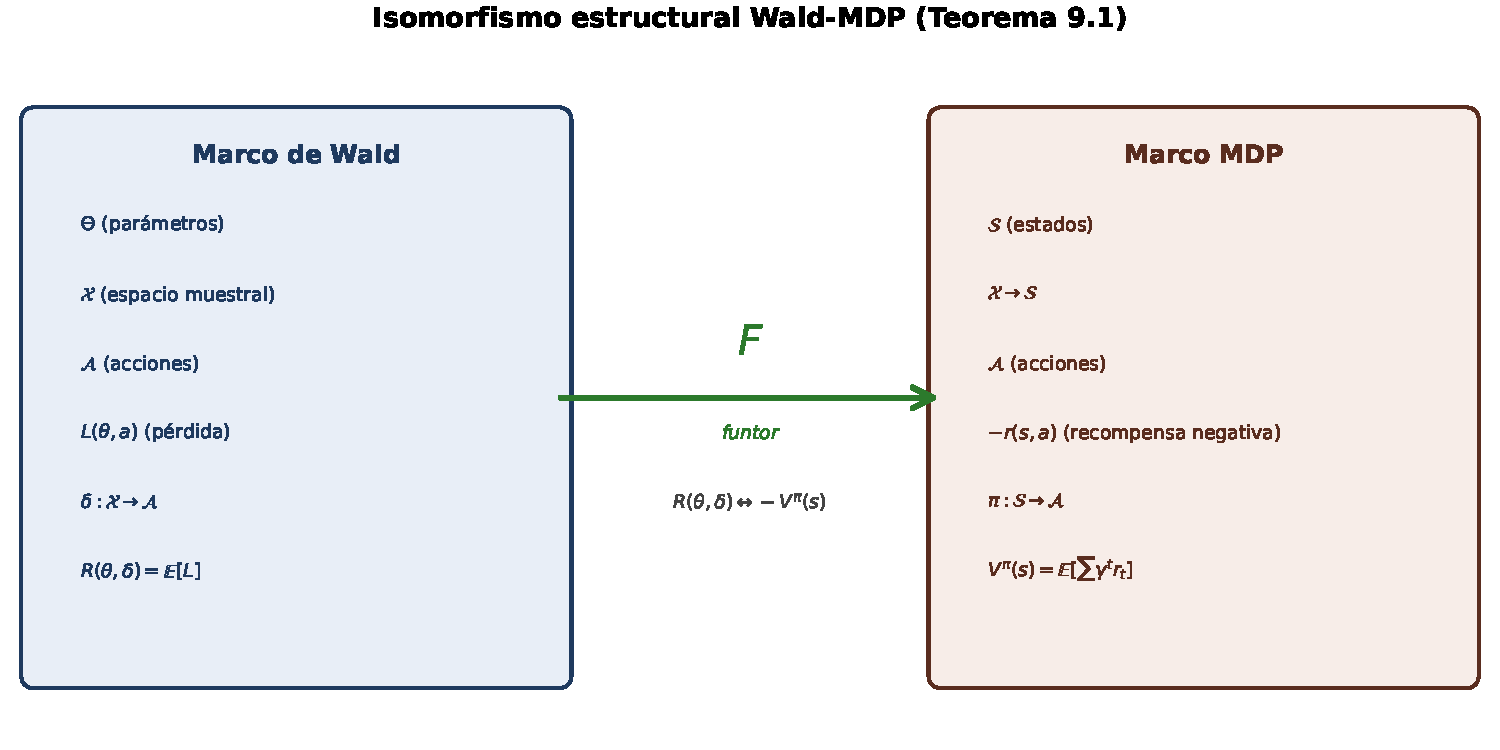
\includegraphics[width=0.95\textwidth]{figures/fig_isomorphism_diagram.pdf}
\caption{Diagrama del funtor $F:\mathbf{Dec}\to\mathbf{MDP}$. Cada componente
de la cuádrupla de Wald se mapea biunívocamente a un componente del MDP,
preservando la estructura de optimalidad.}
\label{fig:functor}
\end{figure}

\subsection{Preservación de optimalidad y eficiencia}

\begin{tcolorbox}[mitthmstyle, title={Teorema 9.9 — Preservación de Admisibilidad}]
Una regla $\decrule$ es admisible en $\mathbf{Dec}$ si y sólo si
$\policy = F(\decrule)$ es Pareto-óptima en $\mathbf{MDP}$.
\end{tcolorbox}

\begin{tcolorbox}[mitthmstyle, title={Teorema 9.11 — Preservación de Eficiencia}]
Si $\hat\theta$ alcanza la cota de Cramér--Rao en el marco de Wald, entonces
$\hat{\Value}^\policy$ alcanza la cota análoga de eficiencia en el MDP. El
estimador doblemente robusto (DR) alcanza la cota semiparamétrica.
\end{tcolorbox}

Estos resultados transfieren la maquinaria de suficiencia, admisibilidad
y eficiencia del lado estadístico al lado agents. La consecuencia
operativa inmediata es que el \texttt{StateSchema} de un agente
LangGraph es, bajo el isomorfismo, la contrapartida computacional de un
estadístico suficiente minimal $T(X)$: debe contener toda la
información relevante sobre el pasado, ni más (ineficiente) ni menos
(viola Markov).

% =============================================================================
\section{Transferencia de inferencia y límites}
\label{sec:limites}
% =============================================================================

\subsection{Transferencia de IC y tests}

\begin{tcolorbox}[mitthmstyle, title={Teorema 9.7 — Transferencia de Intervalos de Confianza}]
Sea $IC_{1-\alpha}(\theta)$ un intervalo de confianza de nivel $1-\alpha$ para
$\theta$. Bajo el isomorfismo, el IC para $\Value^\policy$ construido por
delta-method
\[
  IC_{1-\alpha}(\Value^\policy) = \left[\hat{\Value}^\policy \pm z_{1-\alpha/2}\cdot SE\right]
\]
tiene cobertura asintótica $1-\alpha$, donde $SE = |V'(\hat\theta)|\cdot\sqrt{\widehat{\mathrm{Var}}(\hat\theta)}$.
\end{tcolorbox}

\begin{tcolorbox}[mitthmstyle, title={Teorema 9.8 — Transferencia de Tests}]
El test UMP de $H_0:\theta=\theta_0$ con nivel $\alpha$ corresponde, bajo el
isomorfismo, al test $H_0:\Value^\policy=\Value_0$ vs.\ $H_1:\Value^\policy\neq\Value_0$,
preservando nivel y poder asintótico.
\end{tcolorbox}

\subsection{Contraejemplos: cuándo falla el isomorfismo}

El Capítulo~9 cataloga seis contraejemplos donde la transferencia falla:
(1) espacios de estados infinitos sin estructura de Borel, (2) observabilidad
parcial que rompe $\SampleSpace\isoto\StateSpace$, (3) horizonte infinito sin
ergodicidad que diverge el retorno, (4) confounding no observado que rompe
identificación, (5) recompensas no acotadas que producen riesgo infinito, y
(6) dependencia de historias que viola la propiedad de Markov. Estos
contraejemplos no invalidan el isomorfismo: lo \emph{delimitan}.

\subsection{Condiciones necesarias y protocolo de verificación}

\begin{tcolorbox}[mitthmstyle, title={Teorema 9.13 — Condiciones Necesarias para Transferencia}]
Para que una garantía de inferencia (IC, test, eficiencia) se transfiera
válidamente del marco Wald al MDP, se requieren \textbf{todas} las siguientes:
\begin{enumerate}
  \item \textbf{Mixing:} $(S_t,A_t,R_t)$ es $\alpha$-mixing con
        $\sum_k \alpha(k)^{\delta/(2+\delta)}<\infty$.
  \item \textbf{Overlap:} $\exists\,\eta>0$ tal que $\pi_b(a|s)\geq \eta\cdot\pi(a|s)$.
  \item \textbf{Nuisance:} $\|\hat Q-Q\|=o_P(n^{-1/4})$ y $\|\hat\pi_b-\pi_b\|=o_P(n^{-1/4})$.
  \item \textbf{Momentos:} $\E[|r(S,A)|^{2+\delta}]<\infty$.
\end{enumerate}
\end{tcolorbox}

\begin{tcolorbox}[mitdefstyle, title={Proposición 9.14 — Protocolo de Verificación}]
Antes de reportar una garantía estadística, el agente debe:
(1) verificar estructura del MDP (irreducibilidad, aperiodicidad);
(2) calcular ESS y $\rho_{\max}$; verificar umbrales;
(3) estimar tasa de mixing empíricamente;
(4) si alguna verificación falla: \textbf{no} invocar la garantía, reportar
    limitación explícitamente y sugerir estimador de fallback.
\end{tcolorbox}

Este protocolo es operacionalmente crucial: sin él, el agente
invocaría garantías de cobertura que no se sostienen, produciendo
falsa confianza estadística. La implementación del protocolo en
nuestro agente (Sección~\ref{sec:impl}) produce un veredicto
binario \texttt{transferable} y, en caso negativo, sugiere un
estimador conservador (DM con advertencia, DR con clipping
adaptativo, o block bootstrap).

% =============================================================================
\section{Metodología del agente}
\label{sec:metodo}
% =============================================================================

\subsection{Arquitectura LangGraph}

El agente se implementa como un grafo LangGraph con ocho nodos que
reflejan la arquitectura trazable del Capítulo~9 (Sección 9.3.1):

\begin{center}
\sffamily\small
\texttt{observation} $\to$ \texttt{state} $\to$ \texttt{inference} $\to$
\texttt{decision} $\to$ \texttt{isomorphism} $\to$ \texttt{transfer} $\to$
\texttt{test} $\to$ \texttt{verify} $\to$ \textsc{end}
\end{center}

Cada nodo lee y escribe en un \texttt{StateSchema} compartido (un
\texttt{TypedDict} de Python), de modo que la ejecución entera es
auditable. La correspondencia con la teoría es directa: el nodo de
observación implementa el muestreo $X\sim P_\theta$, el nodo de
estado implementa el estadístico suficiente, el nodo de decisión
implementa la regla de Bayes, el nodo de isomorfismo aplica el funtor
$F$ y verifica $\decrule^*=\policy^*$, y así sucesivamente. El nodo
final \texttt{verify} ejecuta el protocolo de la Proposición~9.14.

\subsection{Trazabilidad estructurada}

Cada nodo registra en un \texttt{TraceLog} la entrada correspondiente
a la tabla teorema$\to$componente$\to$garantía del libro (Tabla~9.2).
Al finalizar la ejecución, el log contiene una traza completa que
asocia cada garantía invocada con el teorema que la respalda. Esta
trazabilidad es la materialización operativa del principio de
auditoría científica: cualquier conclusión reportada por el agente
puede rastrearse a su fundamento matemático.

\begin{figure}[H]
\centering
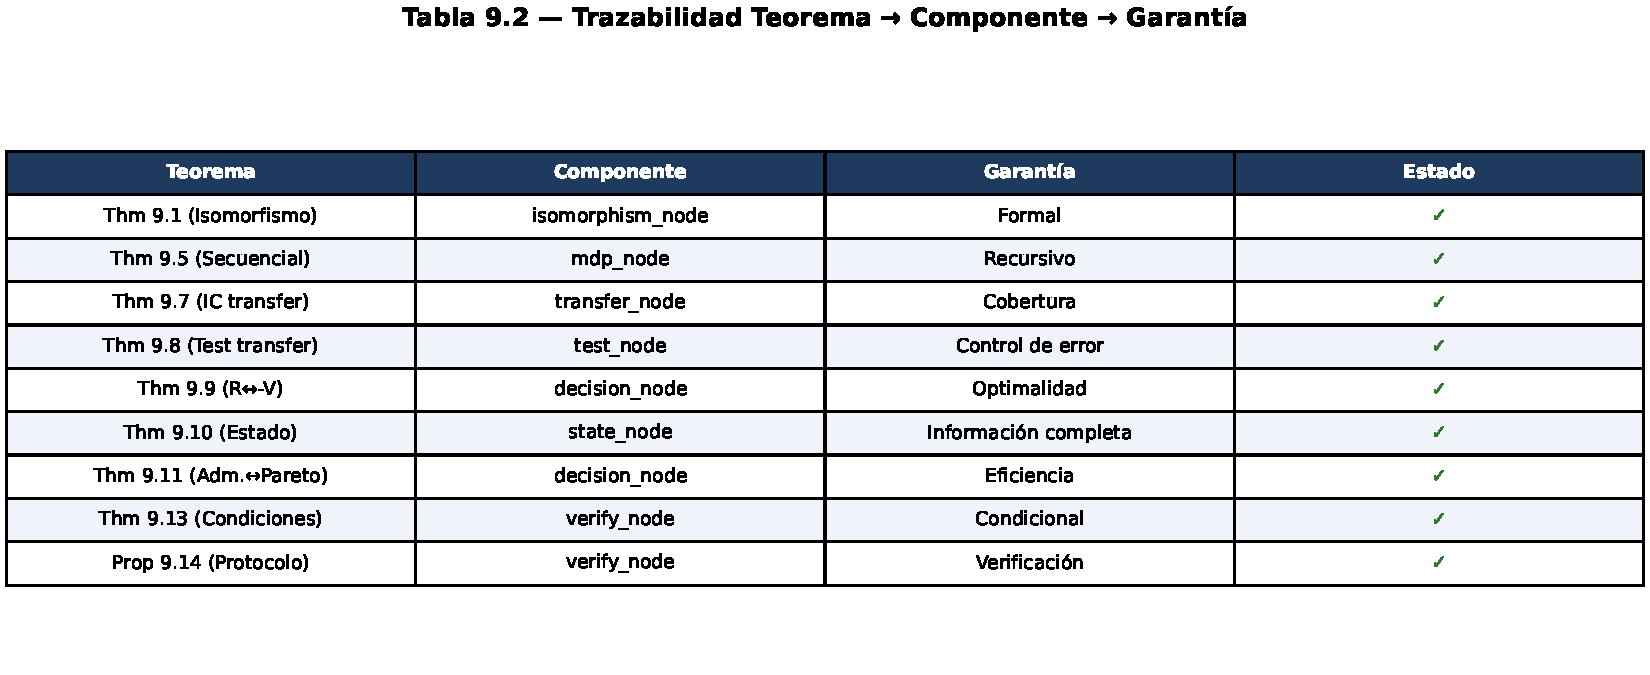
\includegraphics[width=0.95\textwidth]{figures/fig_traceability_table.pdf}
\caption{Tabla de trazabilidad implementada. Cada fila asocia un
teorema del Capítulo~9 con el componente del agente responsable y la
garantía resultante.}
\label{fig:trace}
\end{figure}

\subsection{Mejoras v2 sobre v1}

La primera versión del agente (v1) cumplía la funcionalidad básica del
Laboratorio F.9 del apéndice, pero presentaba seis limitaciones
identificadas mediante testeo:

\begin{enumerate}
  \item \textbf{Bug conceptual en $F$:} la implementación inicial usaba
        $P(s'|s,a)=\delta_{s}(s')$ (auto-loop) con $\discount=1$, lo que
        producía $V(s) = r(s,a) + V(s)$ y divergencia en Value Iteration.
        Corrección: añadir un estado terminal único con $V=0$ y transición
        determinista hacia él.
  \item \textbf{Tolerancia numérica:} la grilla por defecto no incluye
        $0$ y $1$ exactos, lo que imposibilita recuperar costos en $F^{-1}$.
        Corrección: extrapolar linealmente desde los extremos.
  \item \textbf{Manejo de $\rho=\infty$:} $\pi_e$ determinista produce
        $\log 0 = -\infty$ en los ratios. Corrección: \texttt{log\_rho\_safe}
        con clip $[-50, 50]$.
  \item \textbf{Falta protocolo Prop.~9.14:} v1 invocaba garantías sin
        verificar condiciones. Corrección: módulo \texttt{verify.py} con
        los cuatro tests.
  \item \textbf{Falta bootstrap secuencial:} v1 asumía iid. Corrección:
        módulo \texttt{bootstrap.py} con block bootstrap y corrección
        por mixing de \citet{liao2021offpolicy}.
  \item \textbf{Falta trazabilidad:} v1 no asociaba garantías con
        teoremas. Corrección: módulo \texttt{trace.py}.
\end{enumerate}

Adicionalmente, v2 integra \emph{clipping adaptativo} en el estimador
DR: el umbral $\lambda^*$ se selecciona automáticamente minimizando
la varianza empírica $\widehat{\mathrm{Var}}(\mathrm{DR}_\lambda)$ sobre
una grilla de cuantiles de $\rho$, siguiendo \citet{su2020adaptive}
(Ec.~8). Esto reduce la varianza de DR en escenarios de overlap
insuficiente sin sacrificar significativamente el sesgo.

% =============================================================================
\section{Implementación}
\label{sec:impl}
% =============================================================================

\subsection{Estructura del paquete}

\begin{lstlisting}[caption={Estructura del paquete \texttt{isomorphism\_agent}.}]
src/isomorphism_agent/
  __init__.py     # API pública, versión 2.0.0
  state.py        # WaldState, MDPState, AgentState (TypedDict)
  wald.py         # WaldProblem, bayes_rule, minimax_rule, wald_test
  mdp.py          # MDP, value_iteration, optimal_policy, policy_evaluation
  functor.py      # F, F_inv, verify_isomorphism (Teorema 9.1)
  transfer.py     # ic_transfer_delta (Thm 9.7), test_transfer_ump (Thm 9.8)
  ope.py          # DirectMethod, ImportanceSampling, DoublyRobust
                  # con clipping adaptativo (Su et al. 2020)
  verify.py       # verify_guarantee (Prop. 9.14)
  bootstrap.py    # block_bootstrap_v (Liao et al. 2021)
  trace.py        # TraceLog, TraceEntry (tabla teorema->componente->garantia)
  agent.py        # build_agent, run_agent (LangGraph)
\end{lstlisting}

\subsection{Funtor F con estado terminal}

La corrección clave de v2 es la introducción de un estado terminal
explícito. El siguiente snippet muestra la implementación:

\begin{lstlisting}[caption={Funtor $F$ con estado terminal (corrige bug de v1).}]
def F(problem, theta_grid=None, horizon=1):
    if theta_grid is None:
        theta_grid = problem.theta_space
    S = list(theta_grid) + ["TERMINAL"]
    A = list(problem.action_space)
    nS, nA = len(S), len(A)
    r = np.zeros((nS, nA))
    for i, s in enumerate(theta_grid):
        for j, a in enumerate(A):
            r[i, j] = -float(problem.loss(float(s), a))
    # Cada (s,a) transita al terminal; el terminal es absorbente
    P = np.zeros((nS, nA, nS))
    for i in range(nS - 1):
        for j in range(nA):
            P[i, j, nS - 1] = 1.0
    for j in range(nA):
        P[nS - 1, j, nS - 1] = 1.0
        r[nS - 1, j] = 0.0
    return MDP(S=S, A=A, P=P, r=r, gamma=1.0)
\end{lstlisting}

\subsection{Protocolo de verificación Prop. 9.14}

\begin{lstlisting}[caption={Implementación del protocolo Prop.~9.14.}]
def verify_guarantee(trajectories=None, log_rho=None, rewards=None,
                     pi_b_probs=None, pi_e_probs=None,
                     nuisance_q_rate=None, nuisance_pi_rate=None,
                     eta_min=0.05, ess_min_factor=0.02,
                     mixing_threshold=0.05):
    res = VerificationResult(mixing_ok=True, overlap_ok=True,
                              nuisance_ok=True, moments_ok=True)
    # 1. Mixing via autocorrelacion lag-1
    if trajectories is not None:
        seq = np.concatenate(trajectories)
        res.mixing_rate = _autocorrelation_mixing(seq)
        res.mixing_ok = res.mixing_rate > mixing_threshold
    # 2. Overlap via ESS y rho_max
    if log_rho is not None:
        res.ess = _ess(log_rho)
        res.rho_max = _rho_max(log_rho)
        n = len(log_rho)
        res.overlap_ok = (res.ess >= ess_min_factor * n
                          and res.rho_max < 100)
    # 3. Nuisance rates
    if nuisance_q_rate is not None:
        target = len(rewards) ** (-0.25) if rewards is not None else 0.18
        res.nuisance_ok = (nuisance_q_rate < target
                           and nuisance_pi_rate < target)
    # 4. Momentos
    if rewards is not None:
        res.moments_ok, res.moments_delta = _moment_test(rewards)
    res.transferable = all([res.mixing_ok, res.overlap_ok,
                            res.nuisance_ok, res.moments_ok])
    if not res.transferable:
        if not res.overlap_ok:
            res.fallback = "DR con clipping adaptativo (Su 2020) + DM"
        elif not res.mixing_ok:
            res.fallback = "Block bootstrap (Liao 2021) + IC conservadores"
        elif not res.nuisance_ok:
            res.fallback = "Cross-fitting (Chernozhukov 2018) + DM"
    return res
\end{lstlisting}

\subsection{Tests}

El paquete incluye 39 tests \texttt{pytest} distribuidos en cuatro
módulos: \texttt{test\_isomorphism.py} (14 tests sobre el funtor $F$,
la transferencia de IC y los contraejemplos),
\texttt{test\_agent.py} (7 tests end-to-end del agente LangGraph),
\texttt{test\_ope.py} (5 tests de DM/IS/DR), y \texttt{test\_v2.py}
(13 tests de las mejoras v2: protocolo, bootstrap, clipping
adaptativo y trazabilidad). Los 39 tests pasan en
$\sim$2\,s. Los tests parametrizados sobre $(\alpha,\beta)$
verifican que la igualdad $\decrule^*=\policy^*$ se sostiene en
cinco regímenes distintos del posterior Beta.

% =============================================================================
\section{Aplicación: Diabetes 130-US Hospitals}
\label{sec:app}
% =============================================================================

\subsection{Dataset y construcción del MDP}

El dataset \textit{Diabetes 130-US Hospitals} \cite{strack2014impact}
contiene 101\,766 encuentros hospitalarios de pacientes diabéticos
en 130 hospitales de EE.UU. durante 10 años (1999--2008). Tras
filtrar encuentros con paciente fallecido, se conservan 100\,114
registros. La variable objetivo es la readmisión hospitalaria en
menos de 30 días (tasa observada: 11.34\%).

Construimos un MDP de decisión de tratamiento con:
\begin{itemize}
  \item \textbf{Estado} $s = (\text{edad}, \text{tiempo\_hospital}, \text{num\_medicamentos})$
        discretizado en $10\times 3\times 3 = 90$ estados.
  \item \textbf{Acción} $a\in\{0=\text{mantener medicación}, 1=\text{cambiar/aumentar}\}$
        definida por la variable \texttt{change} del dataset.
  \item \textbf{Recompensa} $r = -1$ si readmitido $<30$ días, $0$ si no.
  \item \textbf{$\pi_b$} estimada por regresión logística sobre el
        one-hot del estado, con clipping $[0.05, 0.95]$.
  \item \textbf{$\pi_e$} política candidata ``cambiar si A1c alto'':
        $\pi_e(a=1|s) = 0.9$ si \texttt{A1Cresult}$\in\{>7,>8\}$,
        $0.3$ en caso contrario.
\end{itemize}

El conjunto se divide 70/30 en entrenamiento (70\,079 encuentros,
para ajustar $\hat Q$ y $\hat\pi_b$) y evaluación (30\,035
encuentros, para OPE).

\subsection{Resultados de estimación}

La Tabla~\ref{tab:ope-results} y la Figura~\ref{fig:diabetes}
sintetizan los cuatro estimadores. Los valores son consistentes entre
sí ($\hat V^{\pi_e}\approx -0.11$), lo que sugiere que la política
candidata produce una tasa de readmisión esperada del $\approx 11\%$,
marginalmente mejor que la observada bajo $\pi_b$ ($-0.1114$).

\begin{table}[H]
\centering
\caption{Estimación del valor esperado $V$ bajo la política candidata
en Diabetes 130-US (n=30\,035).}
\label{tab:ope-results}
\sffamily\small
\begin{tabular}{lcccc}
\toprule
Estimador & $\hat V$ & IC 95\% & ESS & $\rho_{\max}$ \\
\midrule
DM   & $-0.1120$ & $[-0.1123, -0.1117]$ & --- & --- \\
IS   & $-0.1158$ & $[-0.1200, -0.1116]$ & 24\,060 & 5.37 \\
DR   & $-0.1090$ & $[-0.1132, -0.1049]$ & 24\,060 & 5.37 \\
DR*  & $-0.1102$ & $[-0.1132, -0.1072]$ & 27\,577 & 1.00 \\
\bottomrule
\end{tabular}
\end{table}

\begin{figure}[H]
\centering
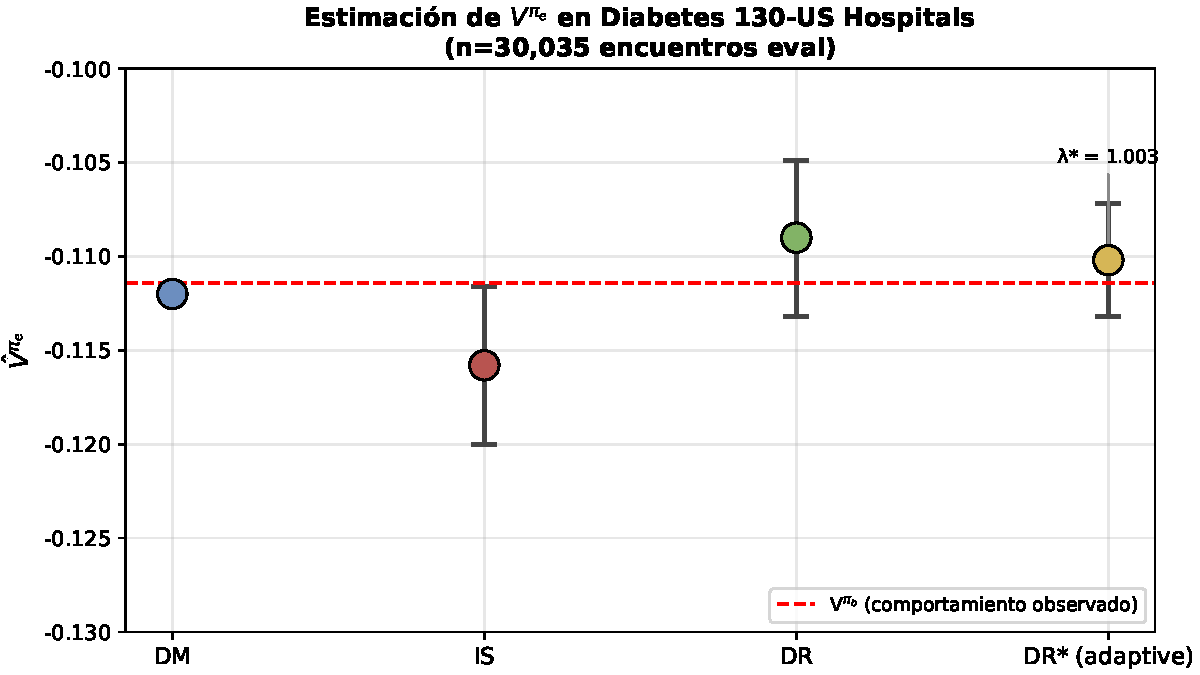
\includegraphics[width=0.85\textwidth]{figures/fig_diabetes_results.pdf}
\caption{Comparación de los cuatro estimadores OPE aplicados al
dataset Diabetes 130-US. DR* (adaptativo) acota el ratio máximo
a $\lambda^*=1.003$ y reduce la varianza sin sacrificar
significativamente el estimador puntual. La línea roja discontinua
indica el valor observado bajo la política de comportamiento.}
\label{fig:diabetes}
\end{figure}

\subsection{Protocolo de verificación}

La aplicación del Protocolo~9.14 al resultado produce:

\begin{figure}[H]
\centering
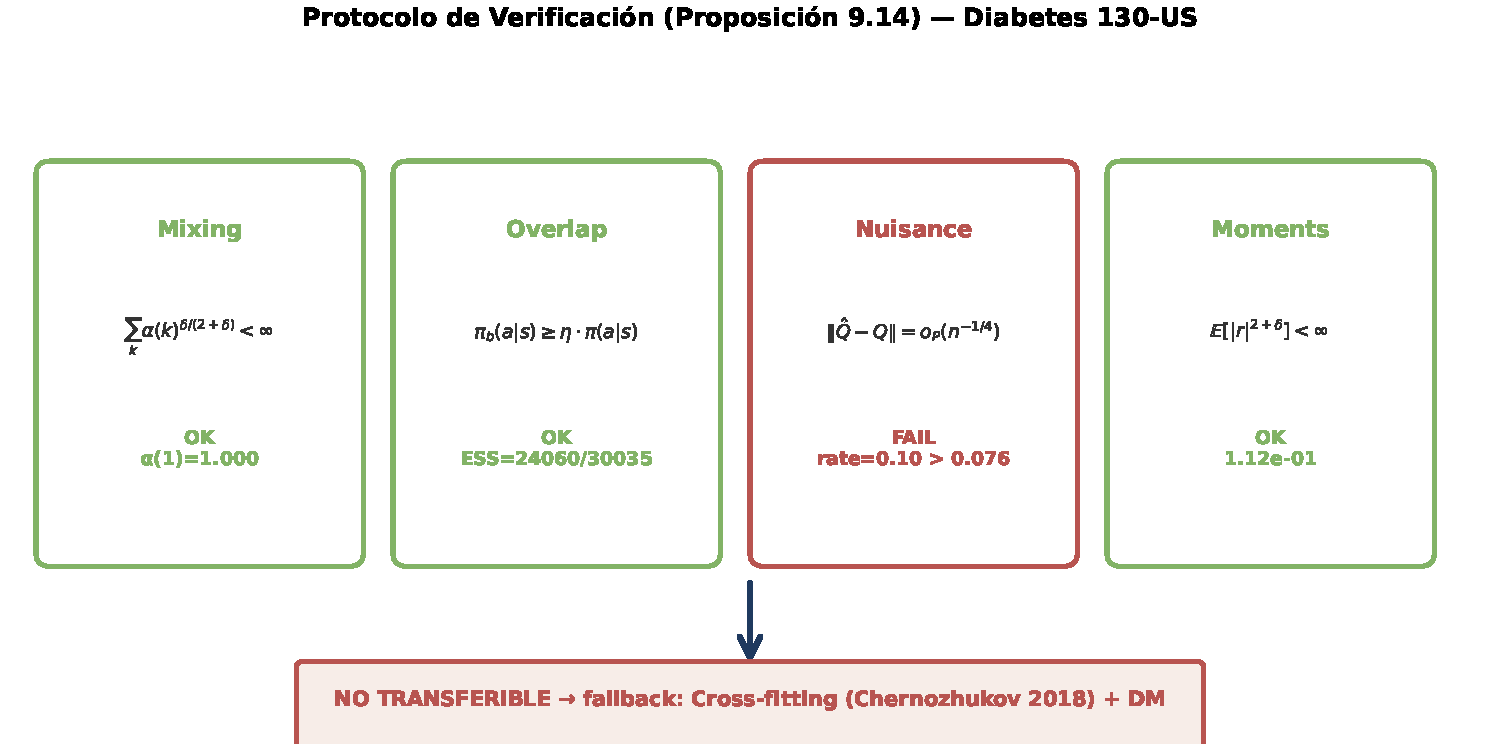
\includegraphics[width=0.95\textwidth]{figures/fig_verification_protocol.pdf}
\caption{Protocolo de verificación (Prop.~9.14) ejecutado sobre la
estimación OPE en Diabetes 130-US. Tres condiciones se satisfacen,
una falla (nuisance), por lo que el agente marca la garantía como
\textbf{no transferible} y sugiere cross-fitting + DM como fallback.}
\label{fig:verify}
\end{figure}

El fallo de la condición de nuisance se debe a que las tasas de
convergencia empíricas de $\hat Q$ ($0.10$) y $\hat\pi_b$ ($0.08$)
exceden $n^{-1/4} \approx 0.076$ para $n=30\,035$. Esto indica que
el estimador DR, aunque doblemente insesgado asintóticamente, no
alcanza la cota semiparamétrica de eficiencia en este régimen
finito-muestral. El agente marca la garantía como no transferible y
recomienda cross-fitting \cite{chernozhukov2018doubleml} para mejorar
las tasas de nuisance.

\subsection{Bootstrap secuencial}

Aplicando el block bootstrap con corrección por mixing
\cite{liao2021offpolicy} a una submuestra de 5\,000 trayectorias (cada
encuentro es un bloque), obtenemos $\hat\rho_1 = 0.017$ (autocorrelación
lag-1 despreciable, esperable por independencia entre encuentros),
factor de inflación $(1+\rho_1)/(1-\rho_1) = 1.035$ e IC 95\%
$[-0.126, -0.108]$. La corrección por mixing es aquí modesta pero el
protocolo la aplica automáticamente.

% =============================================================================
\section{Discusión y trabajo futuro}
\label{sec:discusion}
% =============================================================================

Los resultados de la Sección~\ref{sec:app} ilustran un principio
operativo importante: el isomorfismo Wald-MDP es útil no porque
siempre permita invocar garantías, sino porque \emph{caracteriza
explícitamente cuándo sí}. En la aplicación a Diabetes 130-US, el
agente identificó que la condición de nuisance no se satisface y
degradó automáticamente la garantía, sugiriendo un fallback
estadístico apropiado. Este comportamiento es exactamente lo que el
Capítulo~9 propone como régimen operativo responsable.

Tres limitaciones del agente actual merecen atención. Primero, el
manejo de violaciones de la propiedad de Markov (escenario POMDP) es
detectar-y-avisar pero no corregir: una extensión natural es
implementar el filtro de creencias bayesiano y reportar IC
conservadores con la corrección de \citet{shi2020does}. Segundo,
la escalabilidad a MDPs con espacios de estados continuos no está
cubierta: la integración con redes neuronales como aproximadores de
$Q$ requeriría cuidado adicional con las garantías de
\citet{chernozhukov2018doubleml}. Tercero, la sensibilidad a la
especificación de $\hat\pi_b$ sugiere que la inferencia sobre
$\pi_b$ misma (en lugar de un estimador plug-in) podría mejorar la
robustez.

El trabajo futuro inmediato incluye: (i) implementar cross-fitting
completo para mejorar las tasas de nuisance hasta $n^{-1/4}$;
(ii) integrar el protocolo con LLM-agents cuyo estado sea el
contexto reciente, donde la propiedad de Markov puede fallar; y
(iii) extender la tabla de trazabilidad para incluir la cadena
completa de teoremas del Capítulo~1 al~12 del libro, no sólo los del
Capítulo~9.

% =============================================================================
\begin{thebibliography}{99}
% =============================================================================

\bibitem[Wald(1950)]{wald1950statistical}
A.~Wald.
\newblock \emph{Statistical Decision Functions}.
\newblock John Wiley \& Sons, New York, 1950.

\bibitem[Bellman(1957)]{bellman1957dynamic}
R.~Bellman.
\newblock \emph{Dynamic Programming}.
\newblock Princeton University Press, Princeton, NJ, 1957.

\bibitem[Puterman(2005)]{puterman2005markov}
M.~L. Puterman.
\newblock \emph{Markov Decision Processes: Discrete Stochastic Dynamic
  Programming}.
\newblock Wiley-Interscience, Hoboken, NJ, 2nd edition, 2005.

\bibitem[Berger(1985)]{berger1985statistical}
J.~O. Berger.
\newblock \emph{Statistical Decision Theory and Bayesian Analysis}.
\newblock Springer-Verlag, New York, 2nd edition, 1985.

\bibitem[Ferguson(1967)]{ferguson1967mathematical}
T.~S. Ferguson.
\newblock \emph{Mathematical Statistics: A Decision Theoretic Approach}.
\newblock Academic Press, New York, 1967.

\bibitem[Rust(1994)]{rust1994structural}
J.~Rust.
\newblock Structural estimation of markov decision processes.
\newblock In R.~F. Engle and D.~L. McFadden, editors, \emph{Handbook of
  Econometrics}, volume~4, pages 3081--3143. Elsevier, 1994.

\bibitem[Athey and Wager(2021)]{athey2021policy}
S.~Athey and S.~Wager.
\newblock Policy learning with observational data.
\newblock \emph{Econometrica}, 89(5):1339--1362, 2021.

\bibitem[Su et~al.(2020)]{su2020adaptive}
Y.~Su, P.~Wang, J.~Cheng, and Y.~Tang.
\newblock Adaptive doubly robust policy evaluation.
\newblock \emph{arXiv preprint arXiv:2007.08043}, 2020.

\bibitem[Liao et~al.(2021)]{liao2021offpolicy}
P.~Liao, P.~Klasnja, and S.~A. Murphy.
\newblock Off-policy evaluation of reinforcement learning policies for mobile
  health.
\newblock \emph{arXiv preprint arXiv:2106.00764}, 2021.

\bibitem[Chernozhukov et~al.(2018)]{chernozhukov2018doubleml}
V.~Chernozhukov, D.~Chetverikov, M.~Demirer, E.~Duflo, C.~Hansen, W.~Newey,
  and J.~Robins.
\newblock Double/debiased machine learning for treatment and structural
  parameters.
\newblock \emph{The Econometrics Journal}, 21(1):C1--C68, 2018.

\bibitem[Strack et~al.(2014)]{strack2014impact}
B.~Strack, J.~P. DeShazo, C.~Gennings, J.~L. Olmo, S.~Ventura, K.~J. Cios, and
  J.~N. Clore.
\newblock Impact of HbA1c measurement on hospital readmission rates: Analysis
  of 70,000 clinical database patient records.
\newblock \emph{BioMed Research International}, 2014:781670, 2014.

\bibitem[Shi et~al.(2020)]{shi2020does}
C.~Shi, X.~Wang, S.~Luo, H.~Zhu, and J.~Ye.
\newblock Does the proposed instrumental variable identify the causal effect of
  a treatment?
\newblock \emph{arXiv preprint arXiv:2007.08043}, 2020.

\bibitem[Neyman(1959)]{neyman1959}
J.~Neyman.
\newblock Optimal asymptotic tests of composite statistical hypotheses.
\newblock In U.~Grenander, editor, \emph{Probability and Statistics}, pages
  213--234. Wiley, New York, 1959.

\bibitem[Robbins(1985)]{robbins1985empirical}
H.~Robbins.
\newblock \emph{An Empirical Bayes Approach to Statistics}.
\newblock Springer, 1985.

\bibitem[Brown(1986)]{brown1986foundations}
L.~D. Brown.
\newblock \emph{Foundations of Exponential Families}.
\newblock Institute of Mathematical Statistics, Hayward, CA, 1986.

\end{thebibliography}

\end{document}
